\documentclass{article}

\usepackage{gensymb}
\usepackage{enumitem}
\usepackage{amssymb}
\usepackage{wrapfig}
\usepackage{subfigure}
\usepackage{braket}
\usepackage{amsmath}
\usepackage{graphicx}
\usepackage{mathtools}
\usepackage[letterpaper, margin=1in]{geometry}
\setlength{\parindent}{0cm}

\title{Update on H Elastic Data Analysis - Effect of Extended-Target-Rastered-Beam}
\author{Tritium $(e,e'p)$ Experiment\\Efrain Segarra}
\begin{document}

\maketitle

\textbf{Executive summary:} need to do pointing calibration first, otherwise I'm trying to optimize too many variables with too few equations, and better to first independently constrain the angles. As such, I would reference my other report on pointing calibration. Besides that, I learned a lot of things in this process (mainly to use the rastered beam / extended target corrections), although I think the takeaway is to do pointing properly with our multi-foils for mid kinematics. Between the original report (which showed ($\approx$10-20MeV offsets), and now, is that we realized our scattering angle formula did not match what was stored in the analyzer. Using what was stored in the analyzer allowed better reconstructions overall. However, between extended-target and rastered-beam corrections vs ideal-beam assumptions, the differences are only a couple MeV. 


%%%%%%%%%%%%%%%%%%%%%%%%%%%%%%%%%%%%%%%%%%%%%%%%%%%%%%%%%%%%%%%%%%%%%%%%%%%%%%%%%%%%%%%%%
\section*{Assumptions Made}
First some brief definitions I'll use:
\begin{equation*}
	\begin{gathered}
		p_1^\mu \equiv (E_1,\vec{p}_1)	\textrm{     Electron beam}	\\
		p_2^\mu \equiv (m_p,\vec{0} )	\textrm{     Proton at rest}	\\
		p_3^\mu \equiv (E_3,\vec{p}_3)	\textrm{     Scattered electron}	\\
		p_4^\mu \equiv (E_4,\vec{p}_4)		\textrm{     Scattered proton}
	\end{gathered}
\end{equation*}

Since we are analyzing H data, we are overconstained in what we measure. By just looking at the scattering angles of $\theta_3,\theta_4$, we can determine (1) the beam energy, $E_1$, the scattered electron energy/momentum, $E_3=|\vec{p}_3|$, and (3) the scattered proton energy/momentum, $\vec{p}_4$.\\		

To do so, the first two equations I rederived last night, but originate from a CLAS Collaboration paper by D. Adikaram, et al., ``Towards a resolution of the proton form factor problem: new electron and positron scattering data". The third equation is just conservation of energy-momentum.\\
\begin{equation*}
	\begin{gathered}
		E_1 = m_p ( \cot{\frac{\theta_3}{2}} \cot{\theta_4} - 1 )	\\
		|\vec{p}_3| = E_3 = \frac{ m_p E_1 }{ m_p + E_1 (1-\cos{\theta_3} )}	\\
		|\vec{p}_4| = \sqrt{(E_1 + m_p - E_3)^2 - m_p^2}
	\end{gathered}
\end{equation*}

One can also compare how the reconstructed beam energy looks like under momentum conservation, and see what the resolution is, compared to the angular reconstruction above:
\begin{equation*}
	\begin{gathered}
		E_1 = p_{3} + \sqrt{p_{4}^2 + m_p^2   } -m_p	\\
	\end{gathered}
\end{equation*}

\clearpage

%%%%%%%%%%%%%%%%%%%%%%%%%%%%%%%%%%%%%%%%%%%%%%%%%%%%%%%%%%%%%%%%%%%%%%%%%%%%%%%%%%%%%%%%%
\section*{Cuts Applied}
The cuts I apply are used for all data sets, except of course I don`t include $\theta_{nq}$ cut:
\begin{itemize}
\item{$t_\textrm{coinc} > 10$}
\item{$L_{E/P} >  0.8 $}
\item{$L_{E/P} <  1.3 $}
\item{$|L_z - R_z - 0.005| < 0.02$}
\item{$R_z > -0.1 $}
\item{$R_z < 0.11 $}
\item{$L_z > -0.1 $}
\item{$L_z < 0.11 $}
\item{$|R_\delta| < 0.045 $}
\item{$|L_\delta| < 0.045 $}
\item{$ \left( R_{y\textrm{tar}} + \frac{1.5 R_{y'\textrm{tar}}}{0.08} \right)^2 + \left( \frac{1.5 R_{y'\textrm{tar}}}{0.08} \right)^2 < 1 $}
\item{$ \left( R_{x\textrm{tar}} + \frac{1.5 R_{x'\textrm{tar}}}{0.08} \right)^2 + \left( \frac{1.5 R_{x'\textrm{tar}}}{0.08} \right)^2 < 1 $}
\end{itemize}

%%%%%%%%%%%%%%%%%%%%%%%%%%%%%%%%%%%%%%%%%%%%%%%%%%%%%%%%%%%%%%%%%%%%%%%%%%%%%%%%%%%%%%%%%
\section*{Pre-Optimized Central Values Used}
These are the pre-optimized central kinematic values.
\begin{itemize}
\item{$\theta_e = 17.8018\degree$}
\item{$p_e = 3.54334$ GeV}
\item{$\theta_p = -48.8200\degree$}
\item{$p_p = 1.4805$ GeV}
\end{itemize}


%%%%%%%%%%%%%%%%%%%%%%%%%%%%%%%%%%%%%%%%%%%%%%%%%%%%%%%%%%%%%%%%%%%%%%%%%%%%%%%%%%%%%%%%%
\section*{Results}
First, these are the kinematical distributions that are stored in the skimmed root file (i.e. NOT variables re-calculated based on scattering angles). All of these distributions are produced using the extended-target and rastered-beam corrected variables. \textbf{They also use the scattering angle from the analyzer}.
\begin{center}
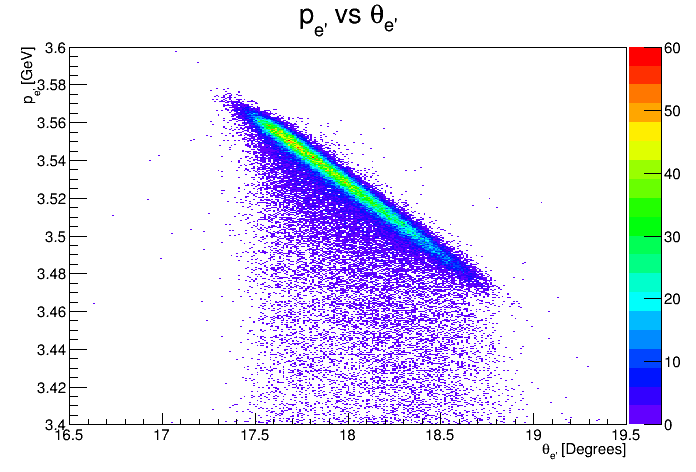
\includegraphics[width=15cm]{Pe_Te.png}\\
Scattered electron angle and momentum.
\end{center}

\begin{center}
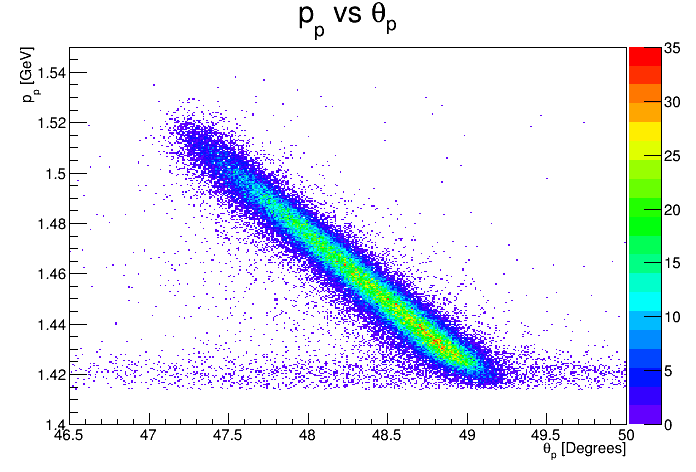
\includegraphics[width=15cm]{Pp_Tp.png}\\
Scattered proton angle and momentum.
\end{center}

\begin{center}
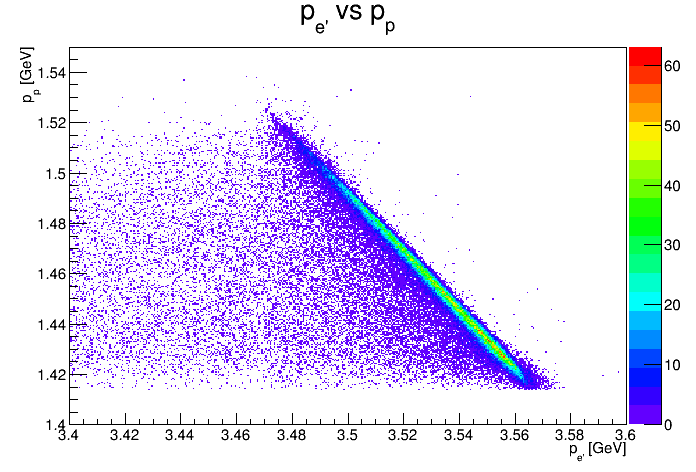
\includegraphics[width=15cm]{Pp_Pe.png}\\
Scattered electron and proton momentum.
\end{center}

\begin{center}
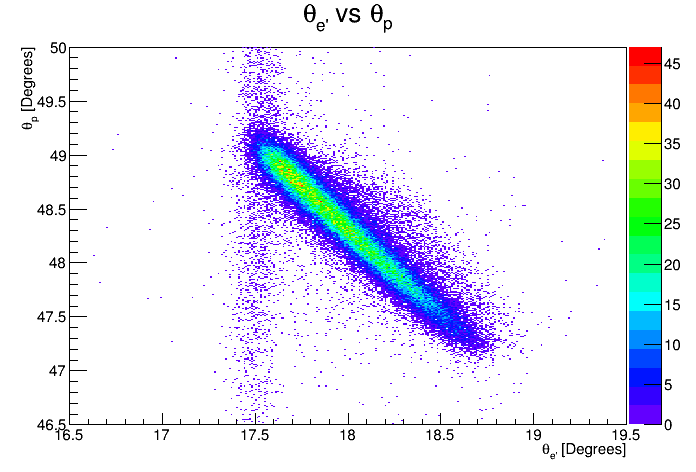
\includegraphics[width=15cm]{Tp_Te.png}\\
Scattered electron and proton angle.
\end{center}

\begin{center}
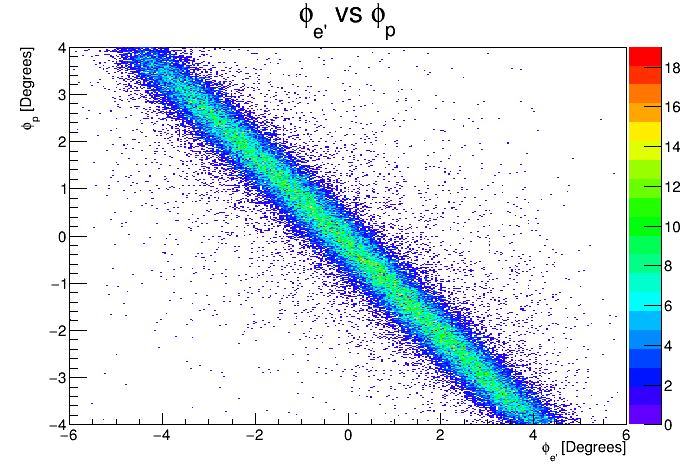
\includegraphics[width=15cm]{DelPhi.png}\\
Scattered electron and proton phi.
\end{center}

\clearpage
Now I looked at the difference between the analyzer scattering angle, and the scattering angle that you can calculate from $y'_{\textrm{tar}} , x'_{\textrm{tar}}$. \textbf{Conclusion:} when comparing the equation-to-analyzer, the two are equivalent for the IDEAL beam case ONLY for the electron. For the proton, there is some odd spread, but it is \textit{roughly} 0. Of course when using extended-target rastered-beam corrections, the two are not equivalent, as they correct for non-ideal beam.

\begin{center}
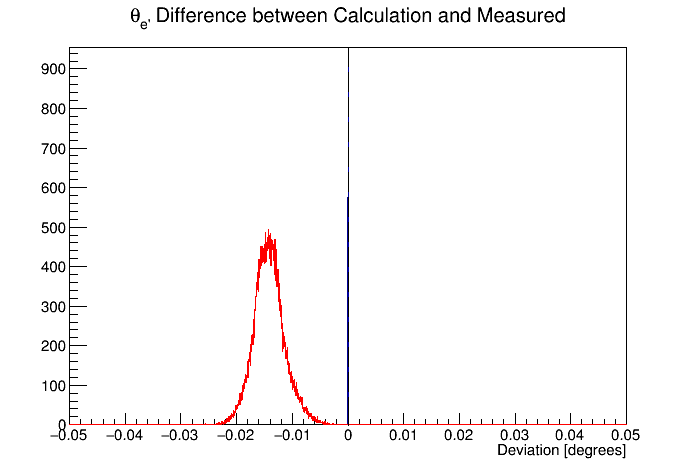
\includegraphics[width=10cm]{thetaDiffe.png}\\
Difference scattering angle for electron (LHRS) between equation and analyzer. The blue is using ideal-beam analyzer variable, the red is using extended-target-rastered-beam analyzer variable. The same equation to calculate the scattering angle is used in both cases. Furthermore, if one uses the \textit{corrected} $y'_{\textrm{tar}} , x'_{\textrm{tar}}$, one still cannot reproduce extended-target-rastered-beam analyzer scattering angle -- they must do some other optimization to extract scattering angle. I also scaled the blue down to show the red curve more clearly.
\end{center}


\begin{center}
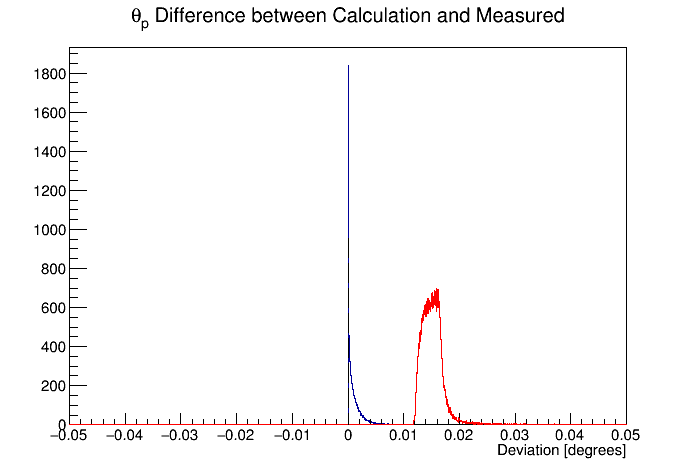
\includegraphics[width=10cm]{thetaDiffp.png}\\
Same as above but for the proton scattering angle. Note here, not even the ideal-beam case is exact. I also scaled the blue down to show the red curve more clearly.
\end{center}

\textbf{The take-away from these two plots means that if we want to ``update" the central angles/momenta of the LHRS, RHRS, we will need to replay all of the files with these corrections, because they do some optimization procedure that we cannot reproduce}. If one wants to calculate a different variable based on scattering angle, one should use their scattering angle, not the equation with corrected $y'_{\textrm{tar}} , x'_{\textrm{tar}}$, as this does not even match what the analyzer outputs.

\clearpage
Now I looked at how much these extended-target-rastered-beam corrections really make a difference in terms of other variables, such as $p_\textrm{miss}$. Summary: they contribute a 1-2 MeV corrections. The offsets seem to be dominated by spectrometer mispointing/misalignment.


\begin{center}
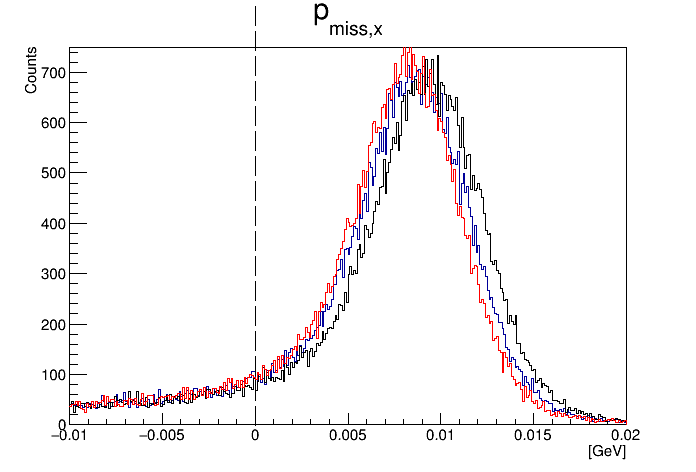
\includegraphics[width=14cm]{Pmx.png}\\
Measured $p_{\textrm{miss},x}$ distributon. The blue curve is assuming ideal beam; the black curve is taking into account rastered-beam corrections; the red curve is taking into account rastered-beam-extended-target corrections.
\end{center}

\begin{center}
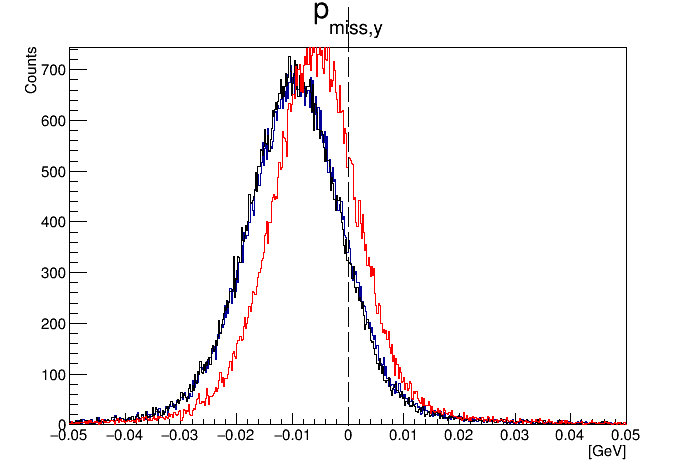
\includegraphics[width=14cm]{Pmy.png}\\
Measured $p_{\textrm{miss},y}$ distributon. The blue curve is assuming ideal beam; the black curve is taking into account rastered-beam corrections; the red curve is taking into account rastered-beam-extended-target corrections.
\end{center}

\begin{center}
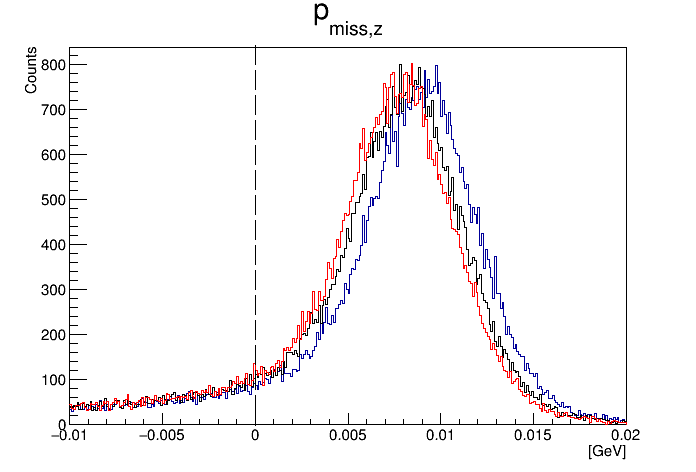
\includegraphics[width=14cm]{Pmz.png}\\
Measured $p_{\textrm{miss},z}$ distributon. The blue curve is assuming ideal beam; the black curve is taking into account rastered-beam corrections; the red curve is taking into account rastered-beam-extended-target corrections.
\end{center}

\begin{center}
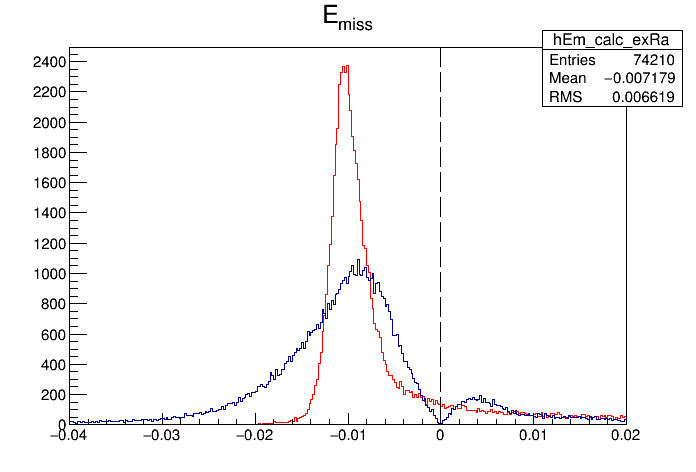
\includegraphics[width=14cm]{Em.png}\\
Measured $E_{\textrm{miss}}$ distributon. The blue curve is from the analyzer, the red curve is what I would reconstruct myself. It seems the analyzer assumes incorrect mass of target, and some sort of inflection around 0? Don`t use analyzer $E_\textrm{miss}$!
\end{center}

\begin{center}
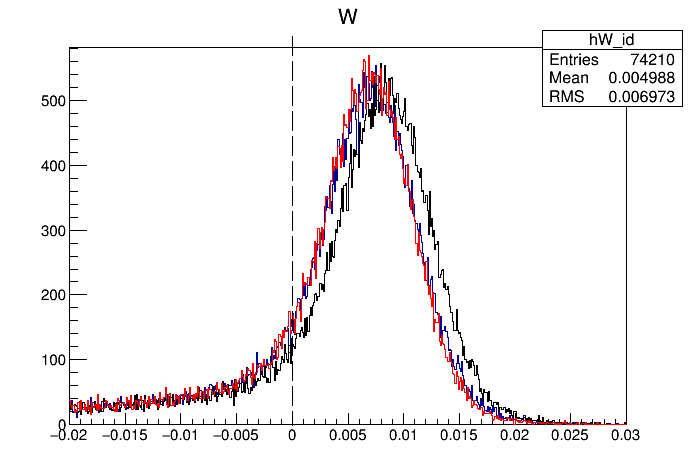
\includegraphics[width=10cm]{delW.png}\\
Difference between measured $W$ distributon and $m_p$. The blue curve is assuming ideal beam; the black curve is taking into account rastered-beam corrections; the red curve is taking into account rastered-beam-extended-target corrections.
\end{center}

\section*{Beam Energy Reconstruction in H(e,e'p)}

Now using the extended-target-rastered-beam scattering angles for LHRS, RHRS, I can reconstruct the beam energy. It seems using angles alone, the spectrum is quite broad, and offset by about 15 MeV, with a FWHM of about 54 MeV. This is comparable to what Paul E. Ulmer and Hassan Ibrahim found in JLAB-TN-00-024, a $10^{-3}$ offset in reconstructed beam energy, when not corrected for spectrometer mispointing. This assumes that the beam energy is known to at least $10^{-4}$, which is to be determined by a more detailed measurement by Doug Higinbotham.\\


\begin{center}
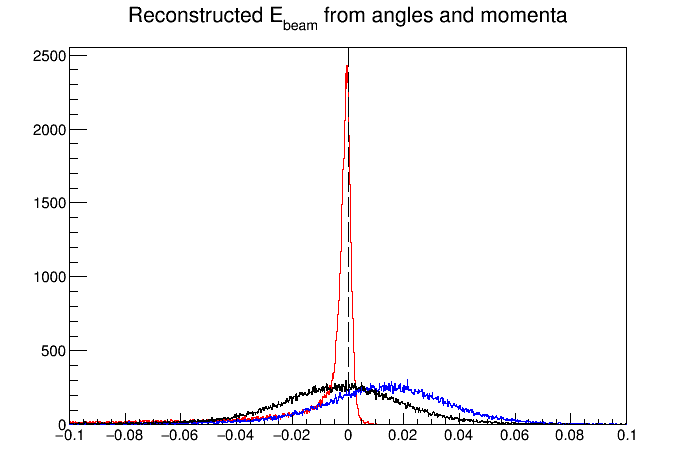
\includegraphics[width=10cm]{delEn2.png}\\
Beam energy reconstructed compared to measured value -- reconstructed from measured momenta (red curve) and reconstructed from measured angles (blue curve). Then, I went through a ``nudging" algorithm to determine the most-probable spectrometer mispointings. This is the black curve. While one might say voila!, this sudo-nudge analysis doesn't exactly fix all the distributions, and it's a bit sketchy. Pointing calibration should independently fix spectrometer angles and not fold in other calibration errors such as momentum.
\end{center}

\textbf{Conclusion: do pointing calibration properly then come back.}






\clearpage





%%%%%%%%%%%%%%%%%%%%%%%%%%%%%%%%%%%%%%%%%%%%%%%%%%%%%%%%%%%%%%%%%%%%%%%%%%%%%%%%%%%%%%%%%




\end{document}
